\section{Riemann and the Reinvention of Integration (1854)}

\subsection{From Waves to Limits: When Fourier Broke the World, Riemann Rebuilt It}

Fourier had shown that functions—even jagged, discontinuous, chaotic ones—could be decomposed into infinite sums of smooth sine waves. This was exhilarating. It was also terrifying. Suddenly, the space of “functions” was not limited to the smooth and sensible—it now included pathological beasts like the square wave and the Dirichlet function.

But there was a catch.

Fourier’s method depended on being able to \emph{integrate} those wild functions. And as mathematicians quickly discovered, classical integration—rooted in intuition and infinitesimals—wasn’t up to the task. For the Dirichlet function, even integration broke down. It wasn’t just hard to compute; it was unclear what “area under the curve” even meant.

Mathematical analysis had reached its breaking point.

\medskip

Enter \textbf{Bernhard Riemann}.

Where Fourier fractured the boundaries of what a function could be, Riemann stepped in to reconstruct the foundations. He didn’t just redefine integration—he reframed what it meant to measure anything at all. 

If functions were going to behave badly, the theory had to grow up.

And Riemann made it rigorous.


\subsection{Riemann Sums: Approximating Area Through Partitions}

Riemann’s key insight was that the \textbf{integral of a function over an interval} could be understood as the limit of finite sums of function values over smaller and smaller partitions of that interval.  

Mathematically, he defined the \textbf{Riemann sum} as:  

\[
S = \sum_{i=1}^{n} f(x_i^*) \Delta x_i
\]

where:  
\begin{itemize}
    \item The interval \([a, b]\) is divided into \textbf{subintervals} \([x_{i-1}, x_i]\), each of width \( \Delta x_i = x_i - x_{i-1} \).  
    \item A representative sample point \( x_i^* \) is chosen from each subinterval.  
    \item The function value at \( x_i^* \) is multiplied by the subinterval width to approximate the area of each strip.  
\end{itemize}

\begin{center}
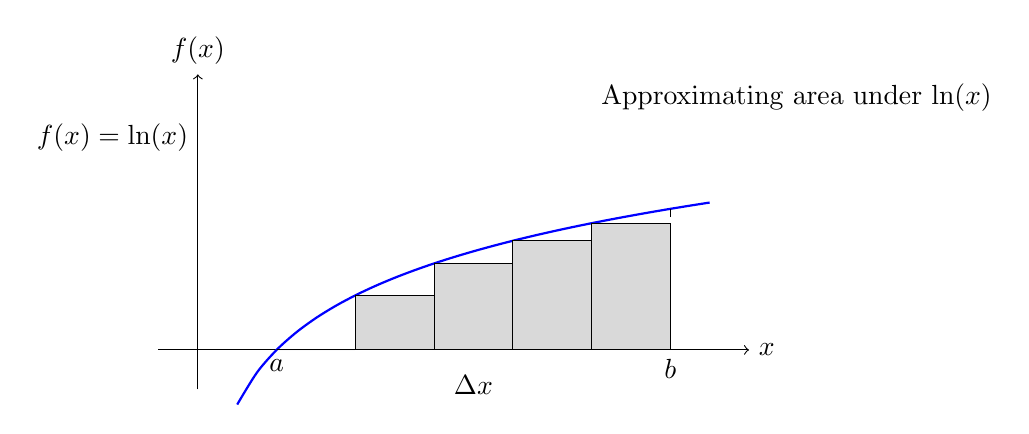
\begin{tikzpicture}
    % Draw axes
    \draw[->] (-0.5,0) -- (7,0) node[right] {\( x \)};
    \draw[->] (0,-0.5) -- (0,3.5) node[above] {\( f(x) \)};
    
    % Function curve: natural logarithm
    \draw[thick, blue, domain=0.5:6.5, smooth] plot (\x, {ln(\x)});
    
    % Interval [a, b]
    \node[below] at (1,0) {\( a \)};
    \node[below] at (6,0) {\( b \)};
    
    % Vertical dashed lines for subintervals
    \foreach \x in {1,2,3,4,5,6} {
        \draw[dashed] (\x,0) -- (\x,{ln(\x)});
    }

    % Rectangles (Riemann sum representation)
    \foreach \x in {1,2,3,4,5} {
        \pgfmathsetmacro\height{ln(\x)}
        \draw[fill=gray!30] (\x,0) rectangle (\x+1,\height);
    }

    % Labels
    \node[below] at (3.5,-0.2) {\( \Delta x \)};
    \node[left] at (0,2.7) {\( f(x) = \ln(x) \)};
    
    % Text description
    \node[right] at (5,3.2) {Approximating area under \( \ln(x) \)};
\end{tikzpicture}
\end{center}


By taking the \textbf{limit as the number of subintervals approaches infinity} (while the width of each subinterval shrinks to zero), the sum converges to a well-defined value—this is the \textbf{Riemann integral}:  

\[
\int_a^b f(x) \,dx = \lim_{n \to \infty} \sum_{i=1}^{n} f(x_i^*) \Delta x_i
\]

This formalization replaced the vague notion of “summing infinitely small quantities” with a \textbf{clear limit process}, ensuring that integration was built on the same solid foundations as differentiation.  







\begin{figure}[H]
\centering
\begin{tikzpicture}
\matrix[matrix of nodes, column sep=1.2cm, row sep=1.2cm] {
% Top-left: 2 rectangles
\node {
  \begin{tikzpicture}[scale=0.6]
    \draw[->] (-0.5,0) -- (7,0) node[right] {\(x\)};
    \draw[->] (0,-0.5) -- (0,3.5) node[above] {\(f(x)\)};
    \draw[thick, blue, domain=1:6.2, smooth] plot (\x, {ln(\x)});
    \foreach \x in {1,3.5} {
        \pgfmathsetmacro\h{ln(\x)}
        \draw[fill=gray!30] (\x,0) rectangle ({\x+2.5}, \h);
    }
    \node at (3,-0.8) {\scriptsize 2 rectangles};
  \end{tikzpicture}
}; &
% Top-right: 3 rectangles
\node {
  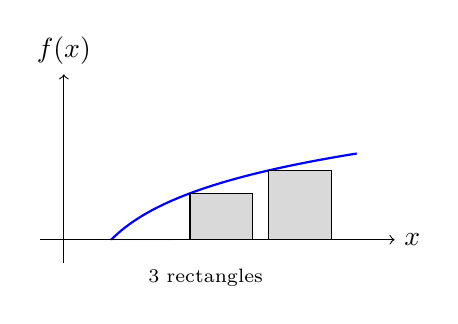
\begin{tikzpicture}[scale=0.6]
    \draw[->] (-0.5,0) -- (7,0) node[right] {\(x\)};
    \draw[->] (0,-0.5) -- (0,3.5) node[above] {\(f(x)\)};
    \draw[thick, blue, domain=1:6.2, smooth] plot (\x, {ln(\x)});
    \foreach \x in {1,2.67,4.33} {
        \pgfmathsetmacro\h{ln(\x)}
        \draw[fill=gray!30] (\x,0) rectangle ({\x+1.33}, \h);
    }
    \node at (3,-0.8) {\scriptsize 3 rectangles};
  \end{tikzpicture}
}; \\
% Bottom-left: 5 rectangles
\node {
  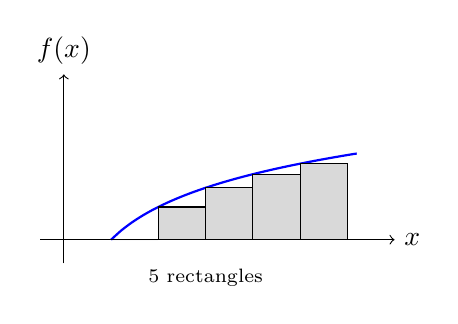
\begin{tikzpicture}[scale=0.6]
    \draw[->] (-0.5,0) -- (7,0) node[right] {\(x\)};
    \draw[->] (0,-0.5) -- (0,3.5) node[above] {\(f(x)\)};
    \draw[thick, blue, domain=1:6.2, smooth] plot (\x, {ln(\x)});
    \foreach \x in {1,2,3,4,5} {
        \pgfmathsetmacro\h{ln(\x)}
        \draw[fill=gray!30] (\x,0) rectangle ({\x+1}, \h);
    }
    \node at (3,-0.8) {\scriptsize 5 rectangles};
  \end{tikzpicture}
}; &
% Bottom-right: 10 rectangles
\node {
  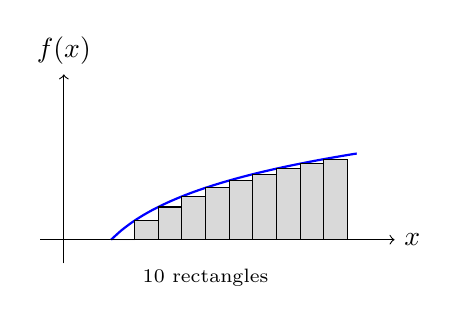
\begin{tikzpicture}[scale=0.6]
    \draw[->] (-0.5,0) -- (7,0) node[right] {\(x\)};
    \draw[->] (0,-0.5) -- (0,3.5) node[above] {\(f(x)\)};
    \draw[thick, blue, domain=1:6.2, smooth] plot (\x, {ln(\x)});
    \foreach \x in {1,1.5,...,5.5} {
        \pgfmathsetmacro\h{ln(\x)}
        \draw[fill=gray!30] (\x,0) rectangle ({\x+0.5}, \h);
    }
    \node at (3,-0.8) {\scriptsize 10 rectangles};
  \end{tikzpicture}
}; \\
};
\end{tikzpicture}
\caption{Left-endpoint Riemann sums: as the number of rectangles increases, the approximation of the area under \( \ln(x) \) becomes more accurate.}
\end{figure}

\subsection{Why Riemann Had to Happen: Taming the Aftermath of Fourier}

Fourier had cracked something open.

When he showed that even a jagged, discontinuous function like the square wave could be written as an infinite sum of smooth sine waves, the mathematical world gasped—then panicked. What did it mean to say that a wild function was “equal” to an infinite trigonometric series? What was being added together? And more pressingly: how do you even integrate something that jumps?

This wasn’t just a philosophical hiccup. Fourier’s method required integration at every turn—to compute coefficients, to reconstruct signals, to make sense of the whole spectral approach. But the functions he summoned weren’t always well-behaved. Many weren’t continuous. Some weren’t even piecewise smooth. The traditional, intuitive tools of calculus buckled under the weight of these constructions.

Enter Riemann.

His approach—defining integration as a limit of sums over partitions—was the perfect antidote. It didn’t rely on smoothness. It didn’t need curves to be gentle. It just needed the function to behave "well enough" on increasingly small intervals. For many of the functions Fourier dealt with, this was just enough structure to bring them back into the realm of the measurable.

\begin{quote}
Where Fourier expanded the space of functions,  
Riemann quietly built the scaffolding to support it.
\end{quote}

Suddenly, it was possible to make sense of integrating a square wave—not because it became smooth, but because Riemann let us sidestep smoothness altogether. The integral was no longer a philosophical notion of accumulated “area,” but a formalized, calculable limit.

And for a time, that limit held.

But as mathematicians dug deeper into Fourier’s zoo of functions, they began to find creatures that slipped even past Riemann’s grasp. Discontinuity was no longer the exception—it was becoming the rule. Some functions didn’t just jump—they shattered every assumption about local structure and convergence.

Riemann had given analysis new ground to stand on.

But just beyond it, the floor was already starting to crack.


\subsection{When Even Riemann Fails: The Dirichlet Function Arrives}

Riemann’s definition of the integral was a triumph of mathematical structure—a way to make sense of wildly misbehaving functions that still held some local order. Where Fourier had cracked open the world of discontinuities, Riemann offered a way to clean up the mess—at least for most of them.

But then came the Dirichlet function.

If the square wave was a rebellious teen testing the limits of classical analysis, the Dirichlet function was a full-blown existential threat.

\[
f_{\text{Dirichlet}}(x) =
\begin{cases}
1, & x \in \mathbb{Q} \\
0, & x \in \mathbb{R} \setminus \mathbb{Q}
\end{cases}
\]

This function is discontinuous \emph{everywhere}. There’s no interval, no neighborhood, no zoom level at which it behaves. It doesn’t spike—it flickers. Rational numbers, being dense, are always nearby. So are irrationals. No matter how small your partition, you’re trapped in a blur of ones and zeros.

And that’s the problem.

Riemann’s method relies on refining partitions: slicing up the interval, choosing representative points, and watching the sums converge. But with the Dirichlet function, there’s no “good” point to pick. Every subinterval is chaos in miniature. Every choice of \(x_i^*\) gives a different answer, and none of them stabilize. The limit simply doesn’t exist.

\begin{quote}
It’s not that the function resists integration.  
It refuses to even be approximated.
\end{quote}

This wasn’t just a mathematical curiosity—it was a full-blown philosophical crisis. The Dirichlet function didn’t just break Riemann’s method; it broke the illusion that all functions could be tamed by clever definitions.

It forced mathematicians to confront an uncomfortable truth:  
not all functions are integrable—even with Riemann’s rigor.

\medskip

And worse: this wasn't the last such function. The 19th century would soon turn into a parade of pathological examples—functions continuous everywhere but differentiable nowhere, limits of convergent series that behaved like statistical hallucinations.

\begin{quote}
Riemann had built a sturdy floor beneath calculus.  
But the Dirichlet function was a trapdoor.
\end{quote}

Soon, someone would open it—and drop us into the abyss.




\subsection{Why the Dirichlet Function Broke Fourier's Approach}

At the heart of Fourier analysis is the idea that a function can be represented as an infinite sum of sine and cosine waves:

\[
f(x) = \frac{a_0}{2} + \sum_{n=1}^{\infty} \left( a_n \cos(nx) + b_n \sin(nx) \right).
\]

where the Fourier coefficients are given by:

\[
a_n = \frac{1}{\pi} \int_{-\pi}^{\pi} f(x) \cos(n x) \,dx, \quad
b_n = \frac{1}{\pi} \int_{-\pi}^{\pi} f(x) \sin(n x) \,dx.
\]

These coefficients describe how much of each frequency contributes to the function’s reconstruction.

To see this in action, consider the square wave:

\[
f(x) = 
\begin{cases}
1, & -\pi < x < 0 \\\\
-1, & 0 < x < \pi
\end{cases}
\quad \text{with } f(-\pi) = f(\pi) = 0
\]

It’s discontinuous, but integrable. Its Fourier series converges to the function almost everywhere:

\[
f(x) \sim \frac{4}{\pi} \left( \sin(x) + \frac{1}{3} \sin(3x) + \frac{1}{5} \sin(5x) + \cdots \right)
\]

\begin{center}
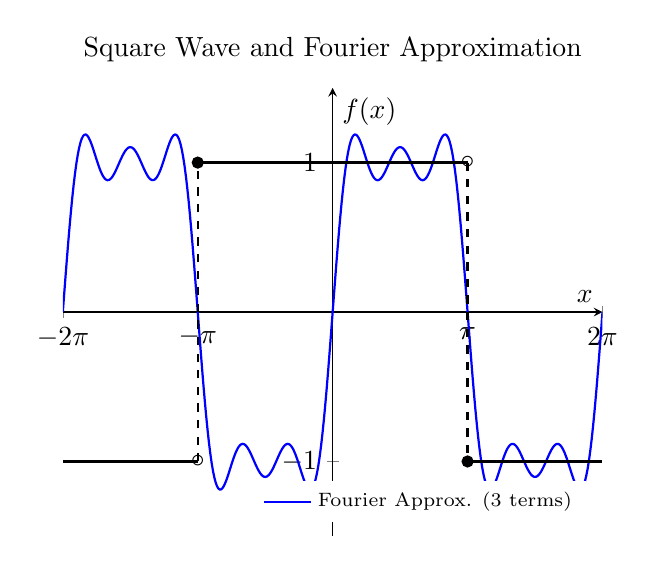
\begin{tikzpicture}
    \begin{axis}[
        domain=-2*pi:2*pi,
        samples=400,
        axis x line=middle,
        axis y line=middle,
        ymin=-1.5, ymax=1.5,
        xlabel={$x$}, ylabel={$f(x)$},
        xtick={-6.28, -3.14, 0, 3.14, 6.28},
        xticklabels={$-2\pi$, $-\pi$, $0$, $\pi$, $2\pi$},
        title={Square Wave and Fourier Approximation},
        legend pos=south east,
        legend style={draw=none, font=\scriptsize}
    ]

        % Fourier approximation (3 sine terms)
        \addplot[blue, thick, domain=-2*pi:2*pi]
        {4/pi*(sin(deg(x)) + 1/3*sin(deg(3*x)) + 1/5*sin(deg(5*x)))};
        \addlegendentry{Fourier Approx. (3 terms)}

        % Square wave segments
        \addplot[black, thick] coordinates {(-2*pi,-1) (-pi,-1)};
        \addplot[black, thick] coordinates {(-pi,1) (pi,1)};
        \addplot[black, thick] coordinates {(pi,-1) (2*pi,-1)};
        
        % Vertical jump lines (discontinuities)
        \addplot[black, thick, dashed] coordinates {(-pi,-1) (-pi,1)};
        \addplot[black, thick, dashed] coordinates {(pi,1) (pi,-1)};

        % Discontinuity markers
        \node at (axis cs: -pi,-1) {\textcolor{black}{$\circ$}};
        \node at (axis cs: pi,1) {\textcolor{black}{$\circ$}};
        \filldraw[black] (axis cs: -pi,1) circle (2pt);
        \filldraw[black] (axis cs: pi,-1) circle (2pt);

    \end{axis}
\end{tikzpicture}
\end{center}


The series does a pretty good job at mimicking the shape, and gets better as we add more terms. Even though the function isn’t differentiable at \( x = 0 \), the Fourier series still works.

\vspace{1em}
\noindent
However, for the Dirichlet function:

\begin{itemize}
    \item It takes values 1 on rationals (a dense but countable set) and 0 on irrationals (an uncountable set).
    \item The Fourier integral sums over both rationals and irrationals.
    \item Since the rationals have measure zero in the traditional sense of Riemann integration, they contribute nothing to the integral.
    \item This results in all Fourier coefficients being zero:
\end{itemize}

\[
a_n = b_n = 0 \quad \forall n.
\]

Which means the Fourier series of the Dirichlet function is just:

\[
f_{\text{Dirichlet}}(x) = 0,
\]

which is clearly wrong. The function does exist, but it defies the assumptions Fourier’s method relies on.

\begin{center}
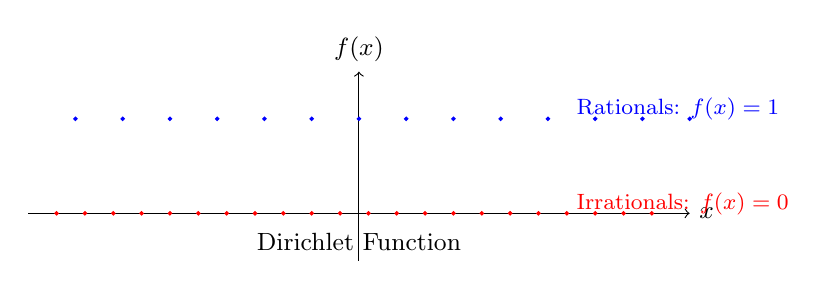
\begin{tikzpicture}[scale=1.2]
  % Axes
  \draw[->] (-3.5, 0) -- (3.5, 0) node[right] {\small $x$};
  \draw[->] (0, -0.5) -- (0, 1.5) node[above] {\small $f(x)$};

  % Dense rational dots at height 1
  \foreach \x in {-3,-2.5,...,3.5} {
    \filldraw[blue] (\x,1) circle (0.5pt);
  }

  % Dense irrational dots at height 0
  \foreach \x in {-3.2,-2.9,...,3.3} {
    \filldraw[red] (\x,0) circle (0.5pt);
  }

  % Labels
  \node[blue, right] at (2.2,1.1) {\footnotesize Rationals: $f(x)=1$};
  \node[red, right] at (2.2,0.1) {\footnotesize Irrationals: $f(x)=0$};
  \node at (0, -0.3) {\small Dirichlet Function};
\end{tikzpicture}
\end{center}

\bigskip

This function revealed a serious limitation of Fourier’s approach: not all functions can be decomposed neatly into sinusoids, especially when they violate our intuitive ideas of smoothness and integrability.


\subsection{When Riemann Breaks: The Crisis of Convergence}

Riemann had rescued integration from the chaos Fourier unleashed. By replacing the vague idea of “infinitely small quantities” with a rigorous limit of sums over partitions, he made the integral precise, predictable, and powerful.

But as mathematics often does, it asked the next uncomfortable question:

\begin{center}
\emph{What happens when even Riemann's rigor isn't enough?}
\end{center}

For all its elegance, the Riemann integral depends on a kind of behavioral decency: that a function behaves “well enough” over small intervals for its sum to stabilize. If we can slice an interval into thinner and thinner subintervals, evaluate the function on each, and let those values add up to something meaningful—great. That’s the integral.

But then came the rebels. Functions that refused to play nice.

These weren’t just sharp or spiky—they were unruly in a deeper sense. On every subinterval, no matter how small, the function could jump, flip, or oscillate without warning. The idea of convergence—the soul of the Riemann sum—evaporated. Sums didn’t stabilize. They danced. They defied reason.

\medskip

This wasn’t just a technicality—it was a philosophical blow.

If integration is supposed to measure “area,” then some functions made measurement meaningless. The more you tried to pin them down, the more they slipped through your fingers. Refining the partition no longer improved the approximation—it just revealed more chaos.

\begin{quote}
The Dirichlet function, for example, was like trying to measure fog with a ruler.
\end{quote}

It forced mathematicians to confront a terrifying possibility:

\begin{center}
\emph{What if not all functions are measurable—not even in Riemann’s sense?}
\end{center}

Mathematics had finally caught up to the implications of its own creations. Fourier had opened the door to infinite decomposition. Riemann tried to contain the madness. But lurking just beyond that containment was something worse: the realization that continuity, reason, and even area could all fail—simultaneously.

\medskip

This wasn’t the end of analysis.

But it was the beginning of a reckoning.

Soon, others would take the stage—not just to refine Riemann’s ideas, but to question everything beneath them. One in particular would detonate what little intuition remained about “smoothness” and “functions.” His name? Let’s just say: you’ll know a monster when you meet one.
